\documentclass[a4paper]{jpconf}
\usepackage{graphicx}
\usepackage{amsmath}

\begin{document}
\title{SWATCH: common control SW for the $\mu$TCA-based upgraded CMS L1 Trigger}

\author{Jim Brooke$^1$, Karol Bunkowski$^2$, Ivan Cali$^3$, Carlos Ghabrous Larrea$^4$, Christos Lazaridis$^4$ and Alessandro Thea$^5$}

\address{$^1$ H.H. Wills Physics Laboratory, University of Bristol, U.K.}
\address{$^2$ Institute of Experimental Physics, University of Warsaw, Poland.}
\address{$^3$ Laboratory for Nuclear Science, Massachusetts Institute of Technology, U.S.A.}
\address{$^4$ Department of Physics, University of Wisconsin-Madison, U.S.A.}
\address{$^5$ Rutherford Appleton Laboratory, STFC, Harwell, U.K.}

\ead{carlos.ghabrous@cern.ch}

\begin{abstract}
The CMS L1 Trigger electronics are composed of a large number of different cards based on the VMEBus standard. The majority of the system is being replaced to adapt the trigger to the higher collision rates the LHC will deliver after the LS1, the first phase on the CMS upgrade program. As a consequence, the software that controls, monitors and tests the hardware will need to be re-written. 
The upgraded trigger will consist of a set of general purpose boards of similar technology that follow the $\mu$TCA specification, thus resulting in a more homogeneous system. A great effort has been made to identify the common firmware blocks and components shared across different cards, regardless of the role they play within the trigger data path. A similar line of work has been followed in order to identify all possible common functionalities in the control software, as well as in the database where the hardware initialisation and configuration data are stored. This will not only increase the homogeneity on the software and database sides, but it will also reduce the manpower needed to accommodate the online SW to the changes on hardware. Due to the fact that the upgrade will take place in different stages, it has been taken into consideration that these new components had to be integrated in the current SW framework. 
This paper presents the design of the control SW and configuration database for the upgraded L1 Trigger. 
\end{abstract}

\section{Introduction}
The L1T (Level-1 Trigger) at the CMS (Compact Muon Solenoid) experiment needs to be adapted to the higher collision rates the LHC will deliver during its second run period \cite{cms_tdr}. The current system, composed by a large number of different electronic cards based on the VMEbus standard, is being replaced by processors based on the telecommunications $\mu$TCA specification \cite{utca_spec}. The reason behind is twofold: in first place, the new design offers an increase in flexibility than that of the current system. This is achieved by using high bandwidth optical links between data cards and larger FPGAs and memory for the trigger logic. In second place, it diminishes the diversity of the hardware ecosystem to a reduced number of general-purpose boards. \\
This upgrade plan encompasses changes in up to 90\% of the existing L1T hardware. Therefore, it is reasonable to expect the redesign of a similar fraction of the firmware, low level software and databases that are used to configure, control and monitor the electronics. As with the hardware, it is planned to pursue a similar path of consolidation on upgrade software, identifying and increasing what is common to all components of the trigger. 

\subsection{The need of a framework to control $\mu$TCA hardware}
The strategy of focusing the development of common online software into a centralised group has led to the conception of the SWATCH (SoftWare for Automating conTrol Common Hardware) project. Its goal is not only to provide a common interface to the new trigger processors exploiting their commonalities. The online software team is also taking the opportunity to provide the L1T community with common high level software components, such as hardware status and monitoring GUIs and test facilities. Although these features are fairly independent on the underlying hardware, at least from an end user point of view, they are elements that had not been provided in the first run of the experiment and each group within the trigger had to develop independently. Furthermore, in the current system the configuration data to setup boards for data taking is stored in databases. Hence, the control software and online databases are coupled to some degree. The project also aims to identify common needs for configuration data storage and proposes a design for an online database schema. 

\subsection{Integration within the current software ecosystem}
Finally, in order to ensure high-efficiency data taking at all times, the upgraded system will be commissioned in parallel with the current system before becoming the baseline for CMS. From the point of view of the control software this means that the new components will have to be integrated with the current control framework, the TS (Trigger Supervisor) \cite{ts_concept}.

\subsection{Organisation of this work}
This paper is organised into seven sections. Section 2 provides a description of the CMS L1 Trigger for runs 1 and 2, pointing out the main differences between the two architectures. Section 3 describes the hardware components that will be part of the upgraded trigger and the efforts to standardise common firmware blocks among them. Sections 4 to 6 present the software and database model designed to control and monitor the $\mu$TCA electronics, discussing as well their integration with the current software framework. Finally, section 7 summarises the work and discusses future developments.

\section{CMS L1T during Run 1 and Run 2}


The CMS L1T is configured, controlled and monitored by its Control and Monitoring Software system. This is a medium-sized distributed system that runs over 40 PCs and 200 processes that control about 4000 electronic boards. The software components of this system are based on the TS framework, written in C++ and providing a web interface using AJAX \cite{ajaxell_lib}. The TS architecture is composed of a hierarchical tree of nodes, where the top node is in charge of coordinating the access to the subsystems. Each node is accessible by a well-defined interface based on the SOAP (Simple Object Access Protocol) \cite{soap_spec}, and can run one or more commands and operations simultaneously. Operations are stateful objects that use transitions to move between different states of their internal finite state machine, while commands are stateless actions taken on the hardware and/or software components. Access to the VME hardware is performed through the VME crate controller and the VME bus using the Hardware Access Library (HAL) \cite{hal_doc}. 

\subsection{Run 2}
The L1T upgrade will bring into the trigger seven new subsystems, over 100 $\mu$TCA boards in three different flavours and around 3000 new optical links to interconnect the new hardware. Unlike VME-based architectures, $\mu$TCA specifications do not specify a hardware access protocol for reading and writing memory spaces from external software applications. This problem has already been solved  through the development of the IPBus suite \cite{ipbus_suite}. A new protocol (IPBus) and hardware access library (uHAL) based on the UDP transport protocol (extensible to TCP and PCI) and C++ language have been developed. The CMS collaboration has agreed on using them as common access methods for hardware configuration and monitoring. Since the hardware control and monitoring commands, translated into IPBus messages, are transported using transport protocols of the internet protocol stack, another configuration of the network has been made possible. This topology favours delocalisation of the control PCs with respect to the hardware, scalability using additional switches and routers and the simplification of PC recovery in case of failure, with the possibility of having redundant computers already connected to the network \cite{tom_paper}.

\section{Hardware processors for the CMS upgraded trigger}

The trigger upgrade is based on $\mu$TCA crates rather than the VME crates used previously in CMS. The $\mu$TCA crate based on the Vadatech VT892 7U chassis \cite{vadatech} is capable of hosting up to 12 AMC modules. Other components that the crate contains are:
\begin{itemize}
  \item $\mu$TCA Carrier Hubs (MCHs); crate management modules that provides Ethernet connection to and from the crate as well as data exchange between AMC cards; 
  \item AMC13, which sits on the second MCH slot of the crate and is the custom module that provides Trigger Timing and Control (TTC) signals, a feedback mechanism for the Trigger Throttling System (TTS) in case data buffers become full, and a high speed link to the Data Acquisition System (DAQ)
\end{itemize}
The diversity of VMEbus-based electronics of the legacy system is being replaced by general-purposed $\mu$TCA boards. These processing cards come in three varieties that are optimised for different tasks: 
\begin{itemize}
  \item CTP7, has dedicated connections to the $\mu$TCA backplane for data sharing within the same crate
  \item MP7, is optimised for data sharing via a large number of optical inputs and outputs
  \item MTF7, is capable of storing large LUT memory resources, which is useful for measurement aspects of the muon trigger. 
\end{itemize}
The three flavours of processors have architectural design differences, but a substantial effort has been taken to extract common functionalities among them and implement them in standard firmware blocks. An abstract model of a trigger upgraded processor is shown in figure 1. 

\begin{figure}
\begin{center}
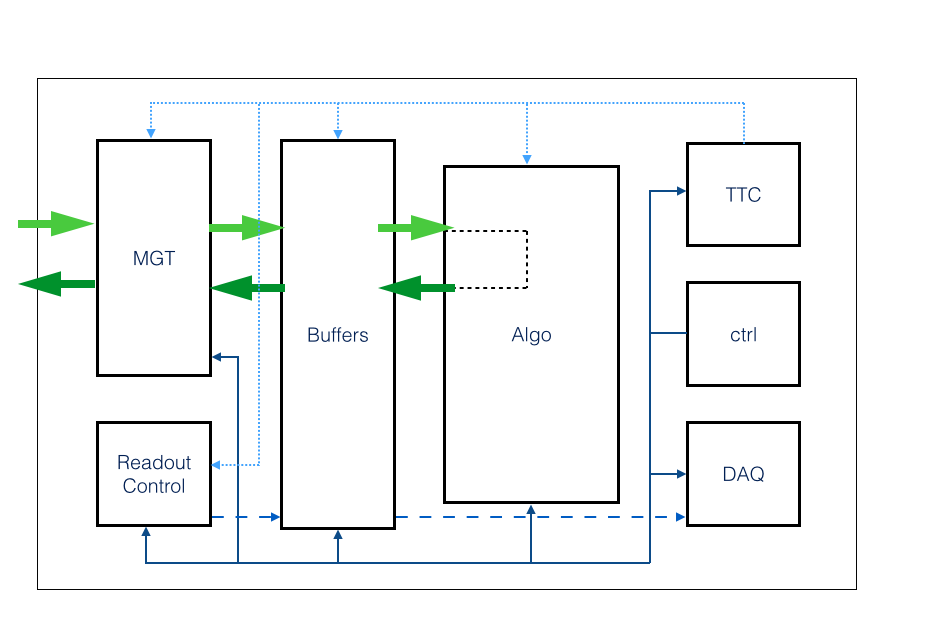
\includegraphics[width=100mm,scale=0.5]{figures/Figure1.png}
\end{center}
\caption{\label{label} Internal firmware blocks of a common processor}
\end{figure}

This flavour-less design of a trigger processor allows to identify the common blocks all processors can share and at the same time leaves flexibility to the firmware designers to allow for custom functionality by implementing the specific behaviour on the algorithm block.


\section{SWATCH control software}

A successful software framework that aims to configure, control and monitor these electronic components must be able to represent them in a generic way. At the same time, it should also leave space for customisation, as developers may need and want to create their own specific actions on these objects. 

%Figure [] shows a simplified version of the initial approach to SWATCH and the classes representing the major hardware components intervening in the trigger upgrade. 
%(figure with device, processor, MP7 and so processors, AMC13 etc). 

Although the heavy use of polymorphism allows objects of specific types to be treated the same way through a common interface, several iterations on the design of SWATCH led to an approach based on composition over inheritance \cite{gof}. The common methods in a class with descendants have been left to a minimum, and the rest of functionalities are contained in different objects of this class. Figure 2 shows the example with the 
\verb Processor  class and their different descendants. 

\begin{figure}
\begin{center}
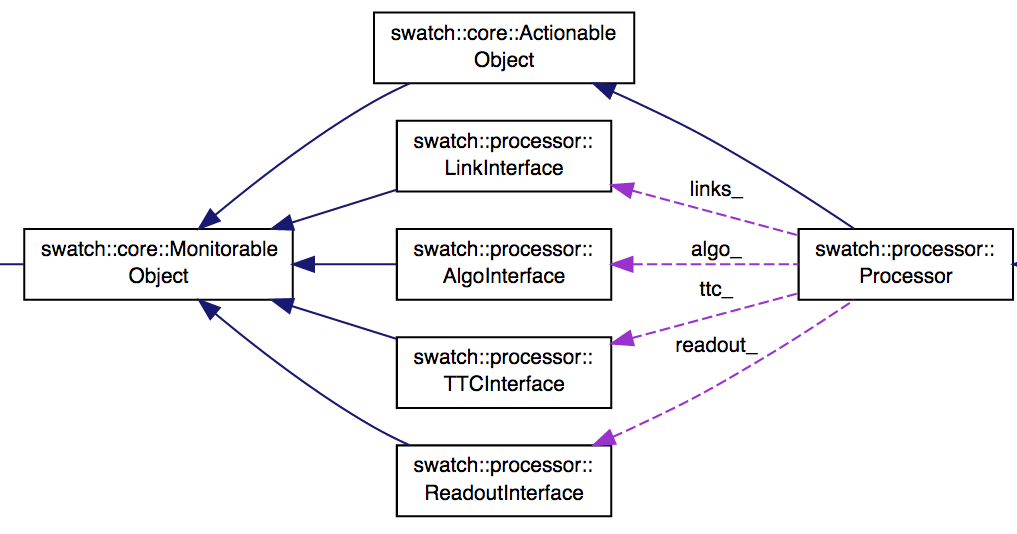
\includegraphics[width=100mm,scale=0.5]{figures/Figure2.png}
\end{center}
\caption{\label{label} The composition of different objects within the Processor class is shown.}
\end{figure}


Composition also plays a major role in the design when it comes to extend the basic functionality of a certain processor type. Instead of allowing the framework user to extend a base class, which might end up with a proliferation of classes that do not necessarily map a certain hardware object anymore, the user can extend commands (stateless) and operations (stateful) to increase and customise the functionality of a hardware item.

\subsection{Package organisation}

The SWATCH package is divided into five main sub packages:

\begin{itemize}
  \item \verb core. Contains the main classes of the SWATCH infrastructure, and base classes representing the different hardware components. Abstract factories have been written that allow the registration of other objects factories, such as System and Processor. Base classes for commands, operations and monitorable objects reside here. 
  \item \verb system. The abstract representation of an upgraded system. The package also maps hardware objects, such as crates and services (MCH, AMC13) in other classes. 
  \item \verb processor. Classes that represent a standard processor for the upgrade and their internal components mapping common firmware blocks.
  \item \verb hardware. Actual concrete classes of hardware items. So far, the MP7Processor and the AMC13Manager classes have been implemented. 
    \item \verb database. Classes that are meant to perform the splitting and distribution of initialisation and configuration data from a permanent storage data source to the hardware components. 
\end{itemize}
    
    The internal structure of the packages has been standardised to facilitate their compilation and distribution through Makefiles and RPMs. Moreover, every package contains a \verb test  subdirectory where unit and functional tests have been implemented using the BOOST test library \cite{boost_test}, thus adopting software quality practices across the new developments. 
    
   
\section{SWATCH common database}

At the L1T configuration data are stored using relational databases. This approach has proved to fulfil the requirements concerning transactions and data persistency. Also, very well defined schemas are necessary to perform the O2O (Online-to-Offline) process, the transfer of information between online and offline databases. Therefore, during the second period of data taking, the L1T will continue with this paradigm and will not adopt other models, such as no relational databases. 

\subsection{Configuration database at the L1T for Run 1}
Configuration data among trigger subsystems has been typically partitioned into different schemas belonging to the different trigger subsystems, with no visibility from one to another. 

%?- how many schemas and tables? How big has the data volume been after run 1?

The design within each subsystem has typically been hierarchical. Figure 3 shows the FK-PK relationships between the master table that contains the configuration for all the trigger subsystems up to the table that hosts the configuration data (values for different registers for one of the boards of a given subsystem).

The \verb GT_GTFE_SETUP  table at the right of the figure holds the configuration of an actual board and illustrates the interdependency between hardware and database tables. 

With such an approach, several areas where the database design could be improved have been identified:
\begin{itemize}
  \item Each register that is written during configuration is represented by a column on this table. This means that if the address table of a board changes (to add a new register, for instance), the table needs to add an extra column. Data already present in the table need to be updated, with the attendant risk of introducing changes to the original data due to a faulty manual intervention. 
  \item Since each trigger group designed their database schema to accommodate it to their specific hardware, the knowledge of the specific designs is distributed over different groups and individuals. This translates into challenges in terms of maintenance and further development, specially taking into account the high manpower turnover within the trigger groups. 
  \item Tables do not contain initialisation data, only configuration. The information the hardware needs to initialise and be brought into a known initial state is distributed at best through RPM packages and more commonly across files within the Network File System, available from all the experiment computers. This situation is far from being ideal, as there is no standard location for initialisation files, nor standard procedures for the hardware to be brought into a ready-to-configure state. 
  \item Finally, configuration data need to be constantly updated by experts at the experiment control room in order to adapt the trigger to operate with different modes (cosmics, pp or heavy ions collisions) and configuration within modes (keys). The L1CE (Level-1 Configuration Editor) is the GUI tool that was developed to allow non database experts to perform such operations, abstracting them from SQL statements needed to insert new configurations on databases. It was also written using the TS as a framework. The maintenance of this tool has proved to be time consuming when it has been necessary to adapt the database infrastructure to new requirements of the upgraded trigger. It is expected that a new tool implemented with more modern web frameworks and more flexible languages will require writing less code to implement the same functionalities and less manpower to maintain it. 

\end{itemize}
   
   
\begin{figure}
\begin{center}
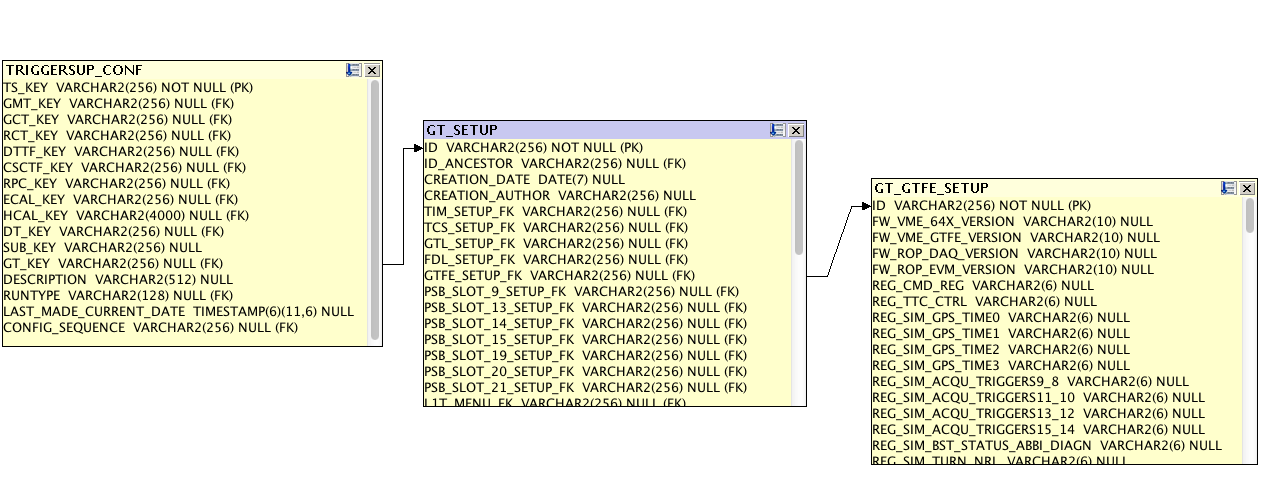
\includegraphics[width=150mm,scale=0.5]{figures/Figure3.png}
\end{center}
\caption{\label{label} FK-PK relationships between the parent configuration table and a board configuration table.}
\end{figure}

    
\subsection {SWATCH database design} 

SWATCH database design follows a radically different approach that tries to solve the problems listed above:

\begin{itemize}
  \item There is only one database schema that hosts the tables for all the trigger subsystem groups. The reason for taking this decision is twofold: on one hand the knowledge, development and maintenance of the database structure is concentrated into a reduced group of experts. On the other, the information and data formats stored in the database are standardised across all trigger subsystems.
  \item This set of tables are divided logically into two groups: one that contains initialisation data, thus hosting quasi-static data, and the other group that stores configuration data. This solves the problem mentioned before: the initialisation data is stored now in a more reliable storage media, and it is also been given standard formats. 
  \item The relation between different tables is partially hierarchical and it is also hardware dependent. A major improvement consists on storing the different hardware configuration items in rows instead of columns, thus avoiding undesired situations when it comes to data updates. All rows whose configuration belongs to the same group or key are tagged with the same identifier. 
  
  %Intermediate table are used where necessary to relate configuration keys with groups of rows that?.?	- 
  
  \item Although these tables have been conceived so that they could store initialisation and configuration data for all the upgraded trigger components, it has also been foreseen a customisation mechanism based on a similar approach of inheritance in OOP, that allows, in case of need, experts to create their own particular tables with customised parameters. 

  \item Finally, to allow experts to edit the database contents and update configurations, a new GUI will be developed. This tool will be based on the GUI used to edit the configuration of the ECAL detector, a successful project that was developed in Python using the minimal framework Flask. By taking the existing GUI as a starting point of development and by using more modern and flexible languages like Python, it is expected  to reduce the development time and also the maintenance costs of this tool.

\end{itemize}


\section{Integration with the current software framework}

The L1T software has to provide the means to configure, control, monitor and validate the new hardware and software components during the commissioning phase while preserving the correct functioning of the legacy trigger. Therefore, the new software packages described previously will have to co-exist with the TS framework. It would also be negligent not to take advantage of the solutions that were found in the past to similar problems.  The TS has successfully operated the legacy trigger components during Run 1, and offers necessary interfaces to run control and to the experiment crew in the form of web pages. 

Although the SWATCH packages are continuously evolving, a beta version has already been chosen to be integrated into the current control software and build a demonstrator, the SWATCH cell, as a proof of concept. The key points this demonstrator should fulfil are:

\begin{description}
  \item[Full integration with Run Control operations.] SWATCH shall operate the $\mu$TCA electronics so that they are ready for data taking. This implies following the different states and transitions defined in the Run Control finite state machine. 
  \item[Configuration from files and databases.] Data used to configure processors reside in permanent storage solutions. SWATCH has to be able to receive the bulk of configuration data from these sources using standard queries, break it down into pieces and distribute them to their corresponding components.
  \item[Status and monitoring.] A general panel in which the status of each hardware component (processor, link) is displayed and updated periodically. Also, a more specific view of this panel will show relevant registers and memory spaces from processors. 
  \item[Introspection.] The end user shall know which actions can be taken on which components.
  \item[Stateless and stateful operations.] The capability of issuing commands (stateless) and operations (stateful) actions into hardware and software components shall be available to the end user. In case of stateful operations it shall be possible to build custom finite state machines. 
\end{description}

\section{Conclusions}

The SWATCH software framework and database design are about to be released to the CMS L1T community. Prototypes showing their main functionalities and features have already been written and deployed in test and integration facilities. Its development has been concentrated into a small group of contributors, reducing the manpower necessary to ensure the advancement of the project and its maintenance, and making more agile the implementation of new features and improvement of existing ones, a strong requirement during the commissioning phase of any project. SWATCH is also being integrated into the TS and demonstrators will soon be available as proof of concept. \\
Future lines of work include a Python binding layer to use SWATCH objects from scripts and CLIs, and extensible mechanisms to allow the performance of hardware integration tests in a standard fashion. 


\section*{References}
\begin{thebibliography}{11}

\bibitem{cms_tdr} The CMS collaboration, \emph{"Technical proposal for the upgrade of the CMS detector through 2020"}, CERN, Geneva 2011. CERN-LHCC-2011-006. 

\bibitem{utca_spec} S. Jamieson of Emerson Network Power, Embedded Computing, \emph{"Micro Telecommunications Computing Architecture Short Form Specification"}, Open Modular Computing Standards, 2006.

\bibitem{ts_concept} I. Magrans de Abril, C-E. Wulz, J. Varela, \emph{"Concept of the CMS Trigger Supervisor"}, IEEE Trans. Nucl. Sci. Vol. 53 Nr. 2, 474-483, 2006.
  
\bibitem{ajaxell_lib} I. Magrans de Abril, M. Magrans de Abril, \emph{"Enhancing the User Interface of the CMS Level 1 Trigger Online Software with AJAX"}, 15th IEEE-NPSS Real-Time Conference, 2007.
  
\bibitem{soap_spec} \emph{"Simple Object Access Protocol"}, http://www.w3.org/TR/soap.
  
\bibitem{hal_doc} C. Schwick, \emph{"HAL (Hardware Access Library)"}, http://cmsdoc.cern.ch/~cschwick/software/documentation/HAL/.
  
\bibitem{ipbus_suite} R. Frazier, G. Iles, D. Newbold, and A. Rose, \emph{"Software and firmware for controlling CMS trigger and readout hardware via gigabit Ethernet"}, Physics Procedia 37 (2012) 1892?1899.
  
\bibitem{tom_paper} T. Williams, \emph{"IPbus: A Flexible Ethernet-based Control System for xTCA Hardware"}, TWEPP 2014 - Topical Workshop on Electronics for Particle Physics.
  
\bibitem{vadatech} Vadatech Inc., \emph{?MicroTCA Chassis with 12 double-width AMC slots?}, 2011, (http://www.vadatech.com/files/pdfs/VT892 SpecRev.pdf).
  
\bibitem{gof} E. Gamma, R. Helm, R. Johnson, J. Vlissides, \emph{"Design Patterns: Elements of Reusable Object-Oriented Software"}, Pearson Education, 1994.
  
\bibitem{boost_test} G. Rozental, \emph{"BOOST test library"}, 2001 - 2007, (http://www.boost.org/doc/libs/1\_58\_0/libs/test/doc/html/index.html).

\end{thebibliography}

\end{document}


